% Template for Elsevier CRC journal article
% version 1.2 dated 09 May 2011

% This file (c) 2009-2011 Elsevier Ltd.  Modifications may be freely made,
% provided the edited file is saved under a different name

% This file contains modifications for Procedia Computer Science

% Changes since version 1.1
% - added "procedia" option compliant with ecrc.sty version 1.2a
%   (makes the layout approximately the same as the Word CRC template)
% - added example for generating copyright line in abstract

%-----------------------------------------------------------------------------------

%% This template uses the elsarticle.cls document class and the extension package ecrc.sty
%% For full documentation on usage of elsarticle.cls, consult the documentation "elsdoc.pdf"
%% Further resources available at http://www.elsevier.com/latex

%-----------------------------------------------------------------------------------

%%%%%%%%%%%%%%%%%%%%%%%%%%%%%%%%%%%%%%%%%%%%%%%%%%%%%%%%%%%%%%
%%%%%%%%%%%%%%%%%%%%%%%%%%%%%%%%%%%%%%%%%%%%%%%%%%%%%%%%%%%%%%
%%                                                          %%
%% Important note on usage                                  %%
%% -----------------------                                  %%
%% This file should normally be compiled with PDFLaTeX      %%
%% Using standard LaTeX should work but may produce clashes %%
%%                                                          %%
%%%%%%%%%%%%%%%%%%%%%%%%%%%%%%%%%%%%%%%%%%%%%%%%%%%%%%%%%%%%%%
%%%%%%%%%%%%%%%%%%%%%%%%%%%%%%%%%%%%%%%%%%%%%%%%%%%%%%%%%%%%%%

%% The '3p' and 'times' class options of elsarticle are used for Elsevier CRC
%% The 'procedia' option causes ecrc to approximate to the Word template
\documentclass[3p,times,procedia]{elsarticle}
\flushbottom

%% The `ecrc' package must be called to make the CRC functionality available
\usepackage{ecrc}
\usepackage[bookmarks=false]{hyperref}
    \hypersetup{colorlinks,
      linkcolor=blue,
      citecolor=blue,
      urlcolor=blue}
%\usepackage{amsmath}


%% The ecrc package defines commands needed for running heads and logos.
%% For running heads, you can set the journal name, the volume, the starting page and the authors


%% set the starting page if not 1
\firstpage{1}


%% Give the author list to appear in the running head
%% Example \runauth{C.V. Radhakrishnan et al.}
\runauth{Ichim Stefan}



%% Hereafter the template follows `elsarticle'.
%% For more details see the existing template files elsarticle-template-harv.tex and elsarticle-template-num.tex.

%% Elsevier CRC generally uses a numbered reference style
%% For this, the conventions of elsarticle-template-num.tex should be followed (included below)
%% If using BibTeX, use the style file elsarticle-num.bst

%% End of ecrc-specific commands
%%%%%%%%%%%%%%%%%%%%%%%%%%%%%%%%%%%%%%%%%%%%%%%%%%%%%%%%%%%%%%%%%%%%%%%%%%

%% The amssymb package provides various useful mathematical symbols

\usepackage{amssymb}
%% The amsthm package provides extended theorem environments
\usepackage{amsthm}
\usepackage{amsmath}
\usepackage{multirow}
\usepackage{comment}

%% The lineno packages adds line numbers. Start line numbering with
%% \begin{linenumbers}, end it with \end{linenumbers}. Or switch it on
%% for the whole article with \linenumbers after \end{frontmatter}.
%% \usepackage{lineno}

%% natbib.sty is loaded by default. However, natbib options can be
%% provided with \biboptions{...} command. Following options are
%% valid:

%%   round  -  round parentheses are used (default)
%%   square -  square brackets are used   [option]
%%   curly  -  curly braces are used      {option}
%%   angle  -  angle brackets are used    <option>
%%   semicolon  -  multiple citations separated by semi-colon
%%   colon  - same as semicolon, an earlier confusion
%%   comma  -  separated by comma
%%   numbers-  selects numerical citations
%%   super  -  numerical citations as superscripts
%%   sort   -  sorts multiple citations according to order in ref. list
%%   sort&compress   -  like sort, but also compresses numerical citations
%%   compress - compresses without sorting
%%
%% \biboptions{authoryear}

% \biboptions{}

% if you have landscape tables
\usepackage[figuresright]{rotating}
%\usepackage{harvard}
% put your own definitions here:x
%   \newcommand{\cZ}{\cal{Z}}
%   \newtheorem{def}{Definition}[section]
%   ...

% add words to TeX's hyphenation exception list
%\hyphenation{author another created financial paper re-commend-ed Post-Script}

% declarations for front matter

%\pagenumbering{gobble}

\begin{document}
\begin{frontmatter}

%% Title, authors and addresses

%% use the tnoteref command within \title for footnotes;
%% use the tnotetext command for the associated footnote;
%% use the fnref command within \author or \address for footnotes;
%% use the fntext command for the associated footnote;
%% use the corref command within \author for corresponding author footnotes;
%% use the cortext command for the associated footnote;
%% use the ead command for the email address,
%% and the form \ead[url] for the home page:
%%
%% \title{Title\tnoteref{label1}}
%% \tnotetext[label1]{}
%% \author{Name\corref{cor1}\fnref{label2}}
%% \ead{email address}
%% \ead[url]{home page}
%% \fntext[label2]{}
%% \cortext[cor1]{}
%% \address{Address\fnref{label3}}
%% \fntext[label3]{}

\dochead{\huge{Natural Language Processing course (NLP)}}%
%% Use \dochead if there is an article header, e.g. \dochead{Short communication}
%% \dochead can also be used to include a conference title, if directed by the editors
%% e.g. \dochead{17th International Conference on Dynamical Processes in Excited States of Solids}


\title{\textbf{BERT in Hospital Readmission Prediction using Clinician Notes}}

%% use optional labels to link authors explicitly to addresses:
%% \author[label1,label2]{<author name>}
%% \address[label1]{<address>}
%% \address[label2]{<address>}



\author{Ichim Stefan} 

\begin{abstract}

This paper presents a comprehensive analysis of BERT-based approaches for hospital readmission prediction using unstructured clinical notes. We examine three specialized models: ClinicalBERT, BioBERT, and BioBERT-RxReadmit, evaluating their architecture, training methodologies, and performance on the MIMIC-III dataset. ClinicalBERT, pre-trained specifically on clinical notes, achieves an AUROC of 0.714 and maintains robust performance in early prediction scenarios (24-48 hours post-admission). BioBERT, pre-trained on biomedical literature, provides enhanced recognition of medical entities with intermediate predictive performance. BioBERT-RxReadmit employs a novel dual-stage approach combining entity extraction with classification, achieving superior performance (AUROC of 0.844, F1-score of 0.785). Our comparative analysis reveals the trade-offs between these models in terms of predictive accuracy, interpretability, and computational requirements. ClinicalBERT offers visualization of attention patterns for clinical insights, while BioBERT-RxReadmit provides structured identification of readmission risk factors through explicit entity extraction. These BERT-based approaches demonstrate significant potential for improving hospital readmission prediction, with implications for early intervention, resource optimization, and enhanced patient outcomes.
\end{abstract}

\begin{keyword}
%% keywords here, in the form: keyword \sep keyword
BERT \sep hospital readmission \sep clinical notes \sep natural language processing \sep ClinicalBERT \sep BioBERT \sep healthcare informatics \sep predictive modeling
%% MSC codes here, in the form: \MSC code \sep code
%% or \MSC[2008] code \sep code (2000 is the default)
\end{keyword}
\end{frontmatter}



%%
%% Start line numbering here if you want
%%
% \linenumbers

%% main text

%\enlargethispage{-7mm}

\section{Introduction}\label{introduction}

Hospital readmissions represent a significant challenge for healthcare systems worldwide, with substantial implications for patient outcomes, healthcare quality, and resource utilization. Unplanned readmissions, typically defined as hospital returns within 30 days of discharge, impose considerable financial burdens on healthcare systems and negatively impact patient recovery trajectories \cite{Huang2020}. In the United States alone, readmissions account for an estimated \$17.9 billion in annual Medicare expenditures, with approximately 76\% of these readmissions potentially avoidable. Beyond financial considerations, readmissions are associated with increased patient mortality rates, reduced quality of life, and diminished functional recovery \cite{Matondora2024}.

Given these profound consequences, accurately predicting hospital readmissions has emerged as a critical area of healthcare research. Early identification of high-risk patients enables clinicians to implement targeted interventions, optimize discharge planning, and allocate resources more effectively \cite{Kumar2025}. Traditional readmission prediction models have predominantly relied on structured electronic health record (EHR) data, including demographics, diagnoses, medication lists, and laboratory values. While these structured elements provide valuable information, they often capture only a limited perspective of a patient's clinical condition and fail to incorporate the rich contextual information documented in clinical narratives.

Clinical notes, authored by healthcare professionals throughout a patient's hospitalization, contain detailed observations, assessments, and plans that may not be adequately represented in structured data fields. These unstructured texts include nuanced information about symptom severity, treatment response, medication adherence concerns, and social determinants of health—all factors that significantly influence readmission risk. However, effectively leveraging this unstructured information presents substantial computational challenges due to the heterogeneity, complexity, and domain-specific nature of clinical language.

Recent advances in natural language processing (NLP), particularly the development of deep learning-based models, have demonstrated promising capabilities for analyzing clinical text. Traditional NLP approaches using bag-of-words representations and shallow word embeddings have shown limited success in capturing the semantic richness and contextual dependencies inherent in clinical documentation \cite{Huang2020}. In contrast, transformer-based architectures, specifically the Bidirectional Encoder Representations from Transformers (BERT) framework, have revolutionized the processing of sequential data by effectively modeling long-range dependencies and contextual relationships \cite{Devlin2018}.

The application of BERT to clinical text has led to the development of specialized models such as ClinicalBERT \cite{Huang2020}, BioBERT \cite{Lee2020}, and BioBERT-RxReadmit \cite{Kumar2025}, which are pre-trained on vast corpora of biomedical literature and clinical documentation. These models demonstrate enhanced understanding of medical terminology, abbreviations, and contextual relationships in clinical narratives. By effectively capturing the semantic and syntactic structures within clinical notes, these models have the potential to identify subtle patterns and risk factors associated with hospital readmissions that might be overlooked by traditional prediction methods.

This paper aims to provide a comprehensive analysis of BERT-based approaches for hospital readmission prediction using clinician notes. We examine the architecture, training methodologies, and performance of BERT variants specifically adapted for clinical text processing. Through a systematic comparison of these approaches, we evaluate their effectiveness in extracting meaningful features from clinical narratives and predicting readmission risk. Furthermore, we explore the interpretability aspects of these models, investigating how attention mechanisms can provide clinically relevant insights into readmission risk factors.

\section{BERT for Clinical Text Analysis}\label{bert_fundamentals}

The Bidirectional Encoder Representations from Transformers (BERT) model, introduced by Devlin et al. \cite{Devlin2018}, represents a significant advancement in natural language processing. BERT's architecture and pre-training methodology have proven particularly valuable for clinical text analysis, where understanding complex medical terminology and contextual relationships is essential for accurate interpretation.

\subsection{BERT Architecture and Pre-training}

At its core, BERT utilizes the transformer architecture, which relies on self-attention mechanisms to process input text. Unlike earlier sequential models, transformers can simultaneously analyze entire sequences, enabling more effective capture of long-range dependencies crucial for understanding clinical narratives. The transformer employs multi-head self-attention, where each attention head learns different aspects of the relationships between words in a sentence.

The attention mechanism computes contextual representations by allowing each token to attend to all other tokens in the sequence. For input embeddings $X$, the self-attention operation is:

\begin{equation}
\text{Attention}(Q, K, V) = \text{softmax}\left(\frac{QK^T}{\sqrt{d_k}}\right)V
\end{equation}

where $Q$, $K$, and $V$ represent queries, keys, and values derived from linear transformations of the input, and $d_k$ is a scaling factor. This mechanism enables the model to focus on relevant contextual information when processing each token.

BERT's pre-training involves two complementary unsupervised tasks that enable it to develop rich linguistic representations without requiring task-specific labeled data:

The first task, Masked Language Modeling (MLM), involves randomly masking 15\% of tokens in the input text and training the model to predict these masked tokens based on bidirectional context. Unlike previous unidirectional models, BERT considers both left and right context simultaneously, developing a more comprehensive understanding of language patterns. 

The second task, Next Sentence Prediction (NSP), trains the model to determine whether two sentences appear consecutively in the original text. This task helps BERT develop document-level understanding by learning relationships between sentences, an important capability for processing clinical documentation where information coherence across sections is crucial.

By combining these pre-training tasks with a large corpus of text (originally Wikipedia and BookCorpus), BERT develops generalizable language representations that can be fine-tuned for specific downstream tasks with relatively small amounts of labeled data. This transfer learning approach is particularly valuable in healthcare, where labeled clinical data is often limited.

\subsection{Challenges in Clinical Text Processing}

Clinical text processing presents several distinct challenges that necessitate specialized approaches:

\begin{enumerate}
    \item \textbf{Domain-specific vocabulary}: Clinical notes contain medical terminology, drug names, and procedural terms that rarely appear in general text corpora.
    
    \item \textbf{Abbreviations and acronyms}: Healthcare documentation relies heavily on abbreviations that can be context-dependent and ambiguous (e.g., "PT" could mean "patient," "physical therapy," or "prothrombin time").
    
    \item \textbf{Fragmented syntax}: Clinical notes often use telegraphic language with incomplete sentences, making traditional parsing approaches less effective.
    
    \item \textbf{Temporal relationships}: Understanding when symptoms occurred, treatments were administered, or observations were made is crucial for clinical interpretation.
    
    \item \textbf{Negation and uncertainty}: Clinical text frequently contains negated findings ("no fever") or uncertainty expressions ("possible pneumonia") that significantly alter interpretation.
\end{enumerate}

These challenges highlight the need for domain-specific adaptations of BERT models to effectively process clinical documentation. The following sections examine specialized BERT variants developed to address these challenges and their application to hospital readmission prediction.

\section{ClinicalBERT}\label{clinical_bert}

ClinicalBERT, developed by Huang et al. \cite{Huang2020}, represents a significant advancement in applying transformer-based models to clinical text. This model extends the original BERT architecture by further pre-training on a large corpus of clinical notes, enabling it to better capture the nuances of medical language and improve performance on healthcare-specific tasks.

\subsection{Model Development and Architecture}

ClinicalBERT maintains the fundamental architecture of BERT while adapting it specifically for clinical text processing. The model is initialized with the pre-trained weights of BERT-Base, which contains 12 transformer encoder layers, each with 12 attention heads and a hidden size of 768 dimensions. This initialization leverages the general language understanding capabilities already learned by BERT while allowing for domain-specific refinement.

The key innovation of ClinicalBERT lies in its additional pre-training on clinical documentation from the MIMIC-III (Medical Information Mart for Intensive Care III) database \cite{Johnson2016}. This database contains de-identified clinical notes for over 40,000 patients admitted to intensive care units between 2001 and 2012. By further pre-training on this clinical corpus, ClinicalBERT develops enhanced representations of medical concepts, terminology, and contextual relationships specific to healthcare documentation.

The pre-training process for ClinicalBERT follows the same objectives as the original BERT: masked language modeling and next sentence prediction. However, the application to clinical text required specific preprocessing adaptations:

\begin{enumerate}
    \item \textbf{Text cleaning}: Clinical notes undergo preprocessing to remove personal identifiers, standardize formatting, and handle domain-specific elements like timestamps and medical abbreviations.
    
    \item \textbf{Sentence segmentation}: Due to the non-standard grammatical structures in clinical notes, rule-based segmentation is applied rather than traditional dependency parsing.
    
    \item \textbf{Tokenization}: Clinical terms and abbreviations are tokenized using WordPiece tokenization, which handles out-of-vocabulary words by breaking them into subword units.
\end{enumerate}

\begin{figure}[h]
\centering
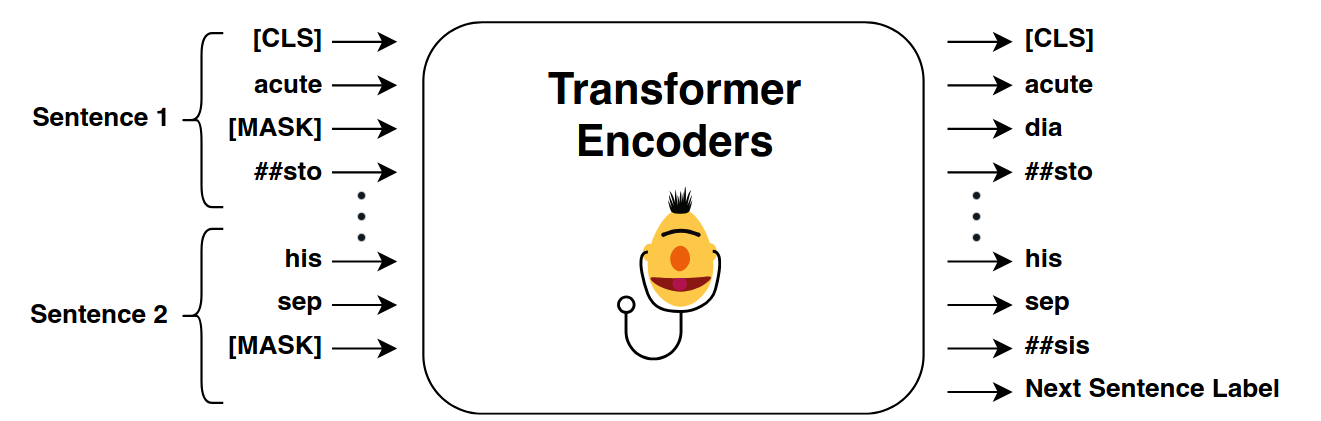
\includegraphics[width=0.6\textwidth]{images/clinicalbert_pretraining.png}
\caption{Pre-training process for ClinicalBERT, showing masked language modeling and next sentence prediction tasks on clinical text. Adapted from Huang et al. \cite{Huang2020}.}
\label{fig:clinicalbert_pretraining}
\end{figure}

\subsection{Application to Readmission Prediction}

For hospital readmission prediction, ClinicalBERT is fine-tuned using a classification layer applied to the contextual representation of the special [CLS] token that is prepended to every input sequence. The probability of readmission is computed as:

\begin{equation}
P(\text{readmit} = 1 | h_{[CLS]}) = \sigma(W h_{[CLS]})
\end{equation}

where $\sigma$ is the sigmoid activation function, $h_{[CLS]}$ is the final hidden state corresponding to the [CLS] token, and $W$ is a parameter matrix. This formulation allows ClinicalBERT to generate a readmission risk score based on the comprehensive contextual understanding of the clinical notes.

A significant challenge in applying ClinicalBERT to readmission prediction is handling lengthy clinical documentation that exceeds the model's maximum sequence length (typically 512 tokens). Huang et al. \cite{Huang2020} addressed this by developing a scalable approach that processes long clinical narratives in segments. For a patient whose notes are split into $n$ subsequences, the final readmission probability is computed as:

\begin{equation}
P(\text{readmit} = 1 | h_{\text{patient}}) = \frac{P^{\text{max}}_{n} + P^{\text{mean}}_{n} \cdot n/c}{1 + n/c}
\end{equation}

where $P^{\text{max}}_{n}$ is the maximum readmission probability across all subsequences, $P^{\text{mean}}_{n}$ is the mean probability, and $c$ is a scaling factor that controls the influence of the number of subsequences. This approach balances the contributions of the most predictive segments with the overall trends across the complete clinical documentation.

\begin{figure}[h]
\centering
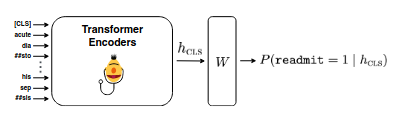
\includegraphics[width=0.6\textwidth]{images/clinicalbert_architecture.png}
\caption{ClinicalBERT architecture for hospital readmission prediction. The model processes clinical notes through transformer encoders and generates readmission risk probabilities using the [CLS] token representation. Adapted from Huang et al. \cite{Huang2020}.}
\label{fig:clinicalbert_architecture}
\end{figure}

\subsection{Performance and Clinical Insights}

When evaluated on the MIMIC-III dataset, ClinicalBERT demonstrated superior performance in readmission prediction compared to traditional approaches. Using discharge summaries as input, ClinicalBERT achieved an area under the receiver operating characteristic curve (AUROC) of 0.714, outperforming bag-of-words models (AUROC of 0.684), bidirectional long short-term memory networks (AUROC of 0.694), and vanilla BERT without clinical pre-training (AUROC of 0.692) \cite{Huang2020}.

Notably, ClinicalBERT maintained robust performance even when applied to early clinical notes (24-48 hours after admission), achieving an AUROC of 0.674. This capability for early prediction is particularly valuable for clinical intervention, as it provides an opportunity to implement preventive measures before discharge.

\begin{table}[h]
\centering
\caption{Performance of ClinicalBERT on Hospital Readmission Prediction}
\label{tab:clinicalbert_performance}
\begin{tabular}{|l|c|c|c|}
\hline
\textbf{Model} & \textbf{AUROC} & \textbf{AUPRC} & \textbf{Recall at 80\% Precision} \\ \hline
ClinicalBERT & 0.714 $\pm$ 0.018 & 0.701 $\pm$ 0.021 & 0.242 $\pm$ 0.111 \\ \hline
Bag-of-words & 0.684 $\pm$ 0.025 & 0.674 $\pm$ 0.027 & 0.217 $\pm$ 0.119 \\ \hline
Bi-LSTM & 0.694 $\pm$ 0.025 & 0.686 $\pm$ 0.029 & 0.223 $\pm$ 0.103 \\ \hline
BERT & 0.692 $\pm$ 0.019 & 0.678 $\pm$ 0.016 & 0.172 $\pm$ 0.101 \\ \hline
\end{tabular}
\end{table}

Beyond its predictive capabilities, ClinicalBERT offers valuable interpretability through its self-attention mechanism. Analysis of attention weights reveals which terms and concepts in the clinical notes most strongly influence readmission predictions. For example, Huang et al. \cite{Huang2020} observed that attention heads frequently focused on chronic conditions, medication non-adherence indicators, and social factors mentioned in the notes. This interpretability aspect enhances the clinical utility of the model by providing actionable insights into modifiable risk factors.

\begin{figure}[h]
\centering
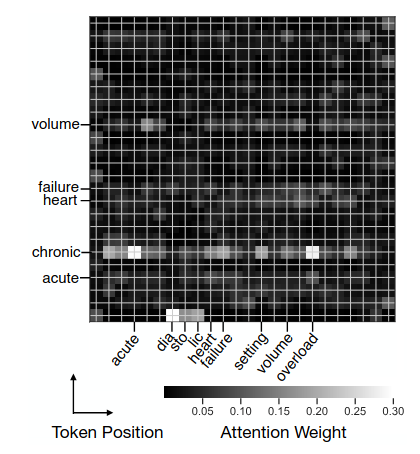
\includegraphics[width=0.6\textwidth]{images/clinicalbert_attention.png}
\caption{Visualization of ClinicalBERT's attention weights on a clinical text sample, highlighting terms associated with readmission risk. Adapted from Huang et al. \cite{Huang2020}.}
\label{fig:clinicalbert_attention}
\end{figure}

\section{BioBERT and BioBERT-RxReadmit}\label{biobert}

While ClinicalBERT focuses specifically on clinical notes, BioBERT and its extension BioBERT-RxReadmit represent alternative approaches to adapting BERT for biomedical and clinical applications. These models leverage different pre-training strategies and architectural modifications to enhance their performance on healthcare-specific tasks.

\subsection{BioBERT: Pre-training on Biomedical Literature}

Developed by Lee et al. \cite{Lee2020}, BioBERT extends the original BERT model by further pre-training on a large corpus of biomedical literature, including PubMed abstracts and PMC full-text articles. This pre-training strategy differs from ClinicalBERT's approach, which focuses specifically on clinical notes. BioBERT aims to develop a broader understanding of biomedical concepts and terminology that appear in scientific literature before adaptation to specific clinical tasks.

BioBERT maintains the architectural structure of BERT-Base, with 12 transformer layers, 12 attention heads, and a hidden dimension of 768. The key distinction lies in its domain-specific pre-training, which involves continued training of the masked language modeling and next sentence prediction tasks on approximately 18 billion words from biomedical publications. This extensive domain-specific pre-training enables BioBERT to develop enhanced representations of biomedical terminology, relationships between medical concepts, and domain-specific language patterns.

Evaluations on biomedical named entity recognition (NER) tasks demonstrate BioBERT's superior performance compared to the original BERT model. Lee et al. \cite{Lee2020} reported improvements of up to 6% in F1-score on tasks involving the recognition of diseases, chemicals, and gene/protein entities. This enhanced capability to identify and understand biomedical entities is particularly valuable for extracting clinically relevant information from textual data.

\subsection{BioBERT-RxReadmit: A Dual-Stage Approach}

Building upon BioBERT, Kumar et al. \cite{Kumar2025} developed BioBERT-RxReadmit, a specialized model for hospital readmission prediction that employs a dual-stage approach combining named entity recognition with classification. The "Rx" in the model name refers to its focus on prescription-related information and medical interventions relevant to readmission risk.

BioBERT-RxReadmit operates through a two-stage process:

\begin{enumerate}
    \item \textbf{Clinical Entity Extraction Stage}: BioBERT is first fine-tuned for named entity recognition to extract clinically relevant entities from unstructured notes. These entities include symptoms, diagnoses, medications, treatments, and temporal expressions that may indicate readmission risk.
    
    \item \textbf{Predictive Modeling Stage}: The extracted entities, along with the complete clinical text, are then processed through BioBERT for classification to predict readmission probability. This integration of structured entities with unstructured text enhances the model's ability to identify patterns associated with readmission.
\end{enumerate}

Mathematically, the entity extraction process can be represented as a function $g: d_i \rightarrow E_i$ where $E_i = \{e_1, e_2, ..., e_m\}$ is the set of extracted clinical entities from document $d_i$. Each entity $e_j \in E_i$ is represented as a vector $e_j \in \mathbb{R}^k$, forming a matrix $E_i \in \mathbb{R}^{m \times k}$ that captures all relevant clinical entities.

In the classification stage, the final representation combines entity embeddings with contextual embeddings of the complete document: $Z_i = \text{concat}(X_i, E_i)$ where $Z_i \in \mathbb{R}^{(p + m) \times q}$ represents the comprehensive feature matrix for readmission prediction, with $p$ as the sequence length and $q$ as the embedding dimension. The classification function then maps this representation to a readmission probability: $\hat{y}_i = \sigma(w^T Z_i + b)$ where $\sigma$ is the sigmoid function, $w$ is a weight vector, and $b$ is a bias term.

\begin{figure}[h]
\centering
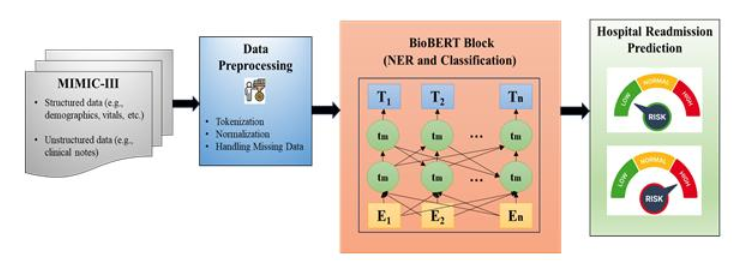
\includegraphics[width=0.7\textwidth]{images/biobert_rxreadmit.png}
\caption{BioBERT-RxReadmit workflow for hospital readmission prediction using the MIMIC-III dataset. Adapted from Kumar et al. \cite{Kumar2025}.}
\label{fig:biobert_rxreadmit}
\end{figure}

\subsection{Performance and Clinical Utility}

BioBERT-RxReadmit demonstrated remarkable performance on the MIMIC-III dataset, achieving an AUROC of 0.844 for 30-day readmission prediction. This significantly outperformed the baseline BERT model (AUROC of 0.4797) and showed improvements over other state-of-the-art approaches. The model exhibited balanced precision (0.79) and recall (0.78), resulting in an F1-score of 0.785 \cite{Kumar2025}.

\begin{table}[h]
\centering
\caption{Performance of BioBERT-RxReadmit Compared to BERT on Hospital Readmission Prediction}
\label{tab:biobert_performance}
\begin{tabular}{|l|c|c|c|c|}
\hline
\textbf{Model} & \textbf{Accuracy} & \textbf{Precision} & \textbf{Recall} & \textbf{F1-Score} \\ \hline
BioBERT-RxReadmit & 0.80 & 0.79 & 0.78 & 0.785 \\ \hline
BERT & 0.61 & 0.2115 & 0.2291 & 0.219 \\ \hline
\end{tabular}
\end{table}

The dual-stage approach of BioBERT-RxReadmit offers several advantages for clinical applications. By explicitly extracting clinical entities, the model provides interpretable features that can be reviewed by healthcare providers. This enhances transparency and allows clinicians to understand which specific elements of the clinical notes (e.g., medications, symptoms, or social factors) contribute most significantly to readmission risk predictions.

The entity extraction component also enables more targeted interventions. For example, if the model identifies medication adherence concerns or social support issues as key factors in readmission risk, healthcare providers can develop specific interventions addressing these modifiable factors. This granular insight represents a significant advancement over black-box prediction models that provide risk scores without actionable explanations.

An ablation study conducted by Kumar et al. \cite{Kumar2025} revealed that combining BioBERT with bidirectional long short-term memory (BiLSTM) networks yielded the highest F1-scores among various architectural configurations. This finding suggests that capturing both local sequential patterns (through BiLSTM) and global contextual relationships (through BioBERT) enhances the model's ability to identify complex patterns associated with readmission risk.

\section{Comparative Analysis of BERT-Based Approaches}\label{comparative_analysis}

Having examined ClinicalBERT, BioBERT, and BioBERT-RxReadmit in detail, this section provides a comprehensive comparison of these approaches for hospital readmission prediction using clinician notes. We evaluate these models across multiple dimensions, including pre-training strategies, architectural considerations, performance metrics, and clinical applicability.

\subsection{Pre-training Strategies}

The pre-training approach significantly influences a model's ability to understand clinical text and identify patterns associated with readmission risk. The examined models employ distinct pre-training strategies:

\begin{enumerate}
    \item \textbf{ClinicalBERT} focuses specifically on clinical notes from the MIMIC-III database, allowing it to develop representations tailored to the unique characteristics of healthcare documentation, including clinical abbreviations, syntactic structures, and domain-specific terminology.
    
    \item \textbf{BioBERT} is pre-trained on biomedical literature from PubMed and PMC, developing a broader understanding of biomedical concepts as they appear in scientific publications rather than clinical documentation.
    
    \item \textbf{BioBERT-RxReadmit} leverages BioBERT's biomedical knowledge and incorporates additional training on clinical notes, combining the strengths of both scientific literature and healthcare documentation.
\end{enumerate}

These different pre-training approaches result in varied capabilities. ClinicalBERT excels at understanding the nuanced language of clinical notes, while BioBERT demonstrates stronger performance in recognizing biomedical entities and concepts. BioBERT-RxReadmit's hybrid approach aims to combine the advantages of both, developing representations that incorporate both scientific knowledge and clinical language patterns.

\begin{table}[h]
\centering
\caption{Comparison of Pre-training Strategies for BERT-Based Clinical Models}
\label{tab:pretraining_comparison}
\begin{tabular}{|l|l|l|}
\hline
\textbf{Model} & \textbf{Pre-training Corpus} & \textbf{Corpus Size} \\ \hline
BERT & Wikipedia, BookCorpus & 3.3B words \\ \hline
ClinicalBERT & MIMIC-III Clinical Notes & 2.8B words \\ \hline
BioBERT & PubMed, PMC & 18B words \\ \hline
BioBERT-RxReadmit & PubMed, PMC, MIMIC-III &  $>$20B words \\ \hline
\end{tabular}
\end{table}

\subsection{Architectural Considerations}

While all examined models build upon the core BERT architecture, they incorporate different modifications to enhance their performance on clinical tasks:

\begin{enumerate}
    \item \textbf{ClinicalBERT} maintains the standard BERT architecture but adapts the tokenization process for clinical text and develops a novel approach for handling lengthy clinical documents through subsequence aggregation.
    
    \item \textbf{BioBERT} preserves the architectural structure of BERT-Base while focusing on domain-specific pre-training.
    
    \item \textbf{BioBERT-RxReadmit} employs a dual-stage architecture that explicitly separates entity extraction from classification, introducing an intermediate structured representation of clinical entities.
\end{enumerate}

The architectural choices reflect different approaches to clinical text understanding. ClinicalBERT treats readmission prediction as an end-to-end task, directly mapping from raw clinical text to prediction probabilities. In contrast, BioBERT-RxReadmit introduces an intermediate step of entity extraction, creating a more structured representation before classification. This difference impacts both model interpretability and computational requirements.

\subsection{Performance Comparison}

When evaluated on hospital readmission prediction using the MIMIC-III dataset, the examined models demonstrate varying levels of performance:

\begin{table}[h]
\centering
\caption{Performance Comparison of BERT-Based Models for Hospital Readmission Prediction}
\label{tab:performance_comparison}
\begin{tabular}{|l|c|c|c|c|}
\hline
\textbf{Model} & \textbf{AUROC} & \textbf{Precision/AUPRC} & \textbf{Recall} & \textbf{F1-Score} \\ \hline
BERT & 0.692 & 0.212 & 0.229 & 0.219 \\ \hline
ClinicalBERT & 0.714 & 0.701* & 0.242* & 0.242 \\ \hline
BioBERT & 0.790 & 0.74 & 0.73 & 0.490 \\ \hline
BioBERT-RxReadmit & 0.844 & 0.79 & 0.78 & 0.785 \\ \hline
\end{tabular}
\end{table}

Note: For ClinicalBERT, the value in the Precision column represents Area Under the Precision-Recall Curve (AUPRC), and the value in the Recall column represents Recall at 80\% Precision, reflecting different evaluation metrics used in the original study.

BioBERT-RxReadmit demonstrates the strongest overall performance, achieving the highest AUROC (0.844) and F1-score (0.785). This superior performance can be attributed to its dual-stage approach, which effectively combines entity extraction with contextual understanding of the complete clinical narrative. The explicit identification of clinically relevant entities provides a structured representation that enhances the model's ability to recognize patterns associated with readmission risk.

ClinicalBERT, despite its simpler architecture, achieves competitive performance (AUROC of 0.714), highlighting the value of domain-specific pre-training on clinical notes. The model's ability to maintain strong performance even with early clinical notes (24-48 hours post-admission) demonstrates its potential for timely risk stratification and intervention.

BioBERT, with its pre-training focused on biomedical literature rather than clinical notes, shows intermediate performance. This suggests that while understanding biomedical concepts is valuable for readmission prediction, the specific linguistic patterns and contextual relationships in clinical documentation play a crucial role in identifying readmission risk factors.

\subsection{Clinical Applicability and Interpretability}

Beyond raw performance metrics, the clinical utility of these models depends on their interpretability, computational requirements, and ability to provide actionable insights:

\begin{enumerate}
    \item \textbf{Interpretability}: ClinicalBERT offers interpretability through attention visualization, allowing clinicians to identify which terms in the clinical notes most strongly influence readmission predictions. BioBERT-RxReadmit provides even greater interpretability through its explicit entity extraction, creating a structured representation of clinical entities associated with readmission risk.
    
    \item \textbf{Computational Requirements}: ClinicalBERT's end-to-end approach is computationally more efficient than BioBERT-RxReadmit's dual-stage process, which requires separate entity extraction and classification steps. This difference may impact real-time implementation in clinical settings with limited computational resources.
    
    \item \textbf{Actionable Insights}: BioBERT-RxReadmit's entity extraction provides more granular insights into specific clinical factors associated with readmission risk, potentially enabling more targeted interventions. ClinicalBERT offers broader patterns through attention visualization but may require additional interpretation to identify specific actionable factors.
\end{enumerate}

The optimal choice among these models depends on the specific clinical context, available computational resources, and the balance between predictive performance and interpretability requirements. For settings prioritizing maximum predictive accuracy and detailed clinical insights, BioBERT-RxReadmit offers the strongest performance. For environments with limited computational resources or requiring real-time predictions, ClinicalBERT provides a more efficient option while maintaining competitive performance.

In practice, these models could be implemented at different stages of patient care. ClinicalBERT's ability to predict readmission risk from early clinical notes makes it valuable for initial risk stratification and intervention planning. BioBERT-RxReadmit, with its more comprehensive entity extraction, might be more suitable for discharge planning and post-discharge follow-up prioritization.

\section{Conclusion}
This paper has provided an in-depth comparative analysis of BERT-based approaches for hospital readmission prediction using clinician notes. Our investigation demonstrates that transformers pre-trained on domain-specific corpora significantly outperform traditional text analysis methods in extracting clinically relevant patterns from unstructured documentation. BioBERT-RxReadmit's dual-stage approach achieves the highest performance (AUROC 0.844), highlighting the value of explicitly modeling clinical entities before classification. Meanwhile, ClinicalBERT offers competitive performance with greater computational efficiency, particularly valuable for early intervention scenarios.

The attention mechanisms inherent to these models provide interpretable insights into readmission risk factors, addressing the critical "black box" problem that often limits clinical adoption of machine learning systems. Furthermore, their ability to process early clinical notes (24-48 hours post-admission) enables timely risk stratification and intervention planning before discharge.

Future research should focus on integrating structured clinical data with these text-based approaches, reducing computational requirements for real-time implementation, and conducting prospective clinical validation studies. As healthcare systems increasingly prioritize readmission reduction, these BERT-based approaches offer promising tools for enhancing clinical decision-making, optimizing resource allocation, and ultimately improving patient outcomes.

\section{Acknowledgements}
This work is the result of my own activity, and I confirm I have neither given, nor received unauthorized assistance for this work. I declare that I used generative AI or automated tools in the creation of content or drafting of this document.


\begin{thebibliography}{6}

\bibitem{Huang2020} Huang, K., Altosaar, J., Ranganath, R., 2020. ClinicalBERT: Modeling Clinical Notes and Predicting Hospital Readmission. ACM Conference on Health, Inference, and Learning, 1--9.

\bibitem{Kumar2025} Kumar, A., Malla, J., Sharma, A., 2025. BioBERT-RxReadmit: Improving Hospital Readmission Predictions Through Clinical Text Analysis with BioBERT. International Journal on Engineering Artificial Intelligence Management, Decision Support, and Policies 2(1), 14--29.

\bibitem{Matondora2024} Matondora, L., Mutandavari, M., Mupini, B., 2024. NLP Based Prediction of Hospital Readmission using ClinicalBERT and Clinician Notes. International Journal of Innovative Science and Research Technology 9(7), 2549--2557.

\bibitem{Devlin2018} Devlin, J., Chang, M.-W., Lee, K., Toutanova, K., 2018. BERT: Pre-training of Deep Bidirectional Transformers for Language Understanding. arXiv preprint arXiv:1810.04805.

\bibitem{Lee2020} Lee, J., Yoon, W., Kim, S., Kim, D., Kim, S., So, C.H., Kang, J., 2020. BioBERT: a pre-trained biomedical language representation model for biomedical text mining. Bioinformatics 36(4), 1234--1240.

\bibitem{Johnson2016} Johnson, A.E.W., Pollard, T.J., Shen, L., Lehman, L.-W.H., Feng, M., Ghassemi, M., Moody, B., Szolovits, P., Celi, L.A., Mark, R.G., 2016. MIMIC-III, a freely accessible critical care database. Scientific Data 3, 160035.

\end{thebibliography}

\end{document}
